% FastVCL -- CVPR 2027 anonymous draft.
% Template status: official CVPR 2027 author kit (v1), downloaded 2026-10-22.
%   archive: https://media.eventhosts.cc/Conferences/CVPR2027/author-kit-CVPR2027-v1-latex.zip
%   archive sha256: 7271bdbb0d2f20043b101c3bb10cba67a8c7f2711f0067b395f9f27451c43121
%   cvpr.sty sha256: 1cd7f434b13d41c475df4a1901a5d82d9ca8b80b8cf6205dc4602a5c164286b4
% The kit dropped the visible Paper ID from the review header; keep this file
% anonymous and do not reintroduce an ID.

\documentclass[10pt,twocolumn,letterpaper]{article}

%%%%%%%%% PAPER TYPE
% \usepackage{cvpr}              % camera-ready
\usepackage[review]{cvpr}      % anonymous review version
% \usepackage[pagenumbers]{cvpr}

% Packages and math macros.  Must be loaded before hyperref.
%% Preamble for the FastVCL CVPR draft.
%% The document class and cvpr.sty are loaded in main.tex; this file only adds
%% packages, math macros and the visible TODO marker.

% The CVPR style selects the legacy Times family. Use its native encoding
% under both pdfLaTeX and XeTeX instead of substituting TU/ptm with another font.
\usepackage[OT1]{fontenc}

% ---------------------------------------------------------------------------
% Layout / tables / algorithms
% ---------------------------------------------------------------------------
\usepackage{array}
\usepackage{multirow}
\usepackage{tabularx}
\usepackage{algorithm}
\usepackage{algpseudocode}
\usepackage{enumitem}
\usepackage{amsthm}

% Algorithm floats inside the two-column text
\renewcommand{\algorithmicrequire}{\textbf{Input:}}
\renewcommand{\algorithmicensure}{\textbf{Output:}}
\floatname{algorithm}{Algorithm}

% Slightly tighter lists
\setlist[itemize]{leftmargin=1.2em,topsep=2pt,itemsep=1pt,parsep=0pt}
\setlist[enumerate]{leftmargin=1.5em,topsep=2pt,itemsep=1pt,parsep=0pt}

% ---------------------------------------------------------------------------
% Visible placeholders.  DO NOT redefine these to be empty: an empty TODO would
% make the draft look finished while the evidence is still outstanding.
% ---------------------------------------------------------------------------
\newcommand{\red}[1]{{\color{red}#1}}
\newcommand{\todo}[1]{{\color{red}#1}}
\newcommand{\TODO}[1]{\textbf{\color{red}[TODO: #1]}}
\newcommand{\PENDING}{\TODO{PENDING}}
\newcommand{\pending}{--}

% ---------------------------------------------------------------------------
% Math notation
% ---------------------------------------------------------------------------
\newcommand{\fA}[1]{\bar{f}^{A}_{#1}}
\newcommand{\fB}[1]{\bar{f}^{B}_{#1}}
\newcommand{\Sim}{S}
\newcommand{\Tube}{\mathcal{T}}
\newcommand{\Anch}{\mathcal{A}}
\newcommand{\Grid}{\mathcal{G}}
\newcommand{\Pred}{\mathcal{P}}
\newcommand{\Step}{\mathcal{S}}
\newcommand{\Track}{\mathcal{I}}
\newcommand{\TopK}{\operatorname{TopK}}
\newcommand{\Dedup}{\operatorname{Dedup}}
\newcommand{\AnchorCap}{\operatorname{Cap}}
\newcommand{\minIoU}{\operatorname{IoU}_{\min}}
\newcommand{\IoU}{\operatorname{IoU}}
\newcommand{\Tloc}{T_{\mathrm{localize}}}
\newcommand{\Taug}{T_{\mathrm{aug}}}
\DeclareMathOperator*{\argmax}{arg\,max}
\DeclareMathOperator*{\argmin}{arg\,min}

% Shorthand for the two video labels (never use them as a batch size)
\newcommand{\vidA}{\mathrm{A}}
\newcommand{\vidB}{\mathrm{B}}

% ---------------------------------------------------------------------------
% Small spacing helpers
% ---------------------------------------------------------------------------
\newcommand{\tabnote}[1]{\par\vspace{-2pt}{\footnotesize #1}}
\setlength{\abovedisplayskip}{4pt}
\setlength{\belowdisplayskip}{4pt}
\setlength{\abovedisplayshortskip}{2pt}
\setlength{\belowdisplayshortskip}{2pt}


\definecolor{cvprblue}{rgb}{0.21,0.49,0.74}
\usepackage[pagebackref,breaklinks,colorlinks,allcolors=cvprblue]{hyperref}

%%%%%%%%% CONFERENCE
\def\confName{CVPR}
\def\confYear{2027}

%%%%%%%%% TITLE
\title{FastVCL: Policy-Guided Dual-Pathway Network for Fast Video Copy Localization}

%%%%%%%%% AUTHORS (suppressed by the review option; kept anonymous on purpose)
\author{Anonymous submission}

\begin{document}
\maketitle

\begin{abstract}
Video Copy Localization (VCL) requires identifying exact temporal boundaries of copied segments across large video collections.
%
Mainstream VCL pipelines rely on dense frame-to-frame correspondence modeling coupled with heavy 2D detectors, which achieves strong accuracy but incurs prohibitive computational overhead when applied uniformly to all video pairs. 
%
In this paper, we propose \textbf{FastVCL}, a fast and adaptive dual-branch VCL framework that dynamically balances localization accuracy and inference efficiency. 
%
Specifically, FastVCL introduces a front-end policy network to assess input samples and route them to either a high-capacity main branch or a lightweight acceleration branch. 
%
For hard or heavily edited pairs, we construct an end-to-end trainable main branch that integrates a frame feature encoder, a learnable similarity matrix, and a 2D object detector for precise boundary localization. 
%
Conversely, regular samples are routed to the acceleration branch, which bypasses heavy detection by directly computing a similarity matrix, extracting anchor candidates, and applying Random Sample Consensus (RANSAC) for rapid temporal alignment.
%
Extensive experiments on standard VCL benchmarks demonstrate that FastVCL achieves competitive localization accuracy on par with state-of-the-art methods while delivering a significant inference speedup.
\end{abstract}
\section{Introduction}
\label{sec:intro}

Video Copy Localization (VCL) aims to identify exact pairs of temporal intervals in which a query video and a reference video share duplicated content. Unlike video-level retrieval, VCL is a fine-grained pairwise localization problem: copied segments frequently undergo severe spatial and temporal transformations—including cropping, picture-in-picture overlays, re-encoding, and playback speed variations—requiring a system to accurately recover both the temporal boundaries and the underlying frame-to-frame alignment~\cite{vcsl2022,transvcl2023}.

To tackle these challenges, state-of-the-art VCL pipelines predominantly adopt a three-stage paradigm comprising a frame feature encoder, a learnable frame-to-frame similarity matrix, and a 2D object detector (or temporal alignment head) operating over the resulting correspondence map~\cite{vcsl2022,transvcl2023}. While applying object detection over dense similarity matrices captures complex temporal patterns with high accuracy, computing and processing full $M \times N$ correspondence maps for video sequences of lengths $M$ and $N$ incurs substantial quadratic overhead. Conversely, sparsifying the similarity matrix via strided anchor matching and band-limited dynamic programming reduces complexity to sub-quadratic levels, but introduces a fundamental precision--recall dilemma. Under a conservative operating point, strict anchor filtering yields high precision on clear copies yet prematurely discards short segments, heavily edited transitions, or weakly matching tracks before localization even begins. Simply relaxing anchor thresholds or densifying the correspondence grid recovers missed copies, but floods the detector with ambiguous false alarms triggered by repetitive textures, static logos, and visually similar background shots.

\begin{figure*}[t]
\centering
% Uncomment the line below in your local CVPR project when figures/framework.pdf is present:
% 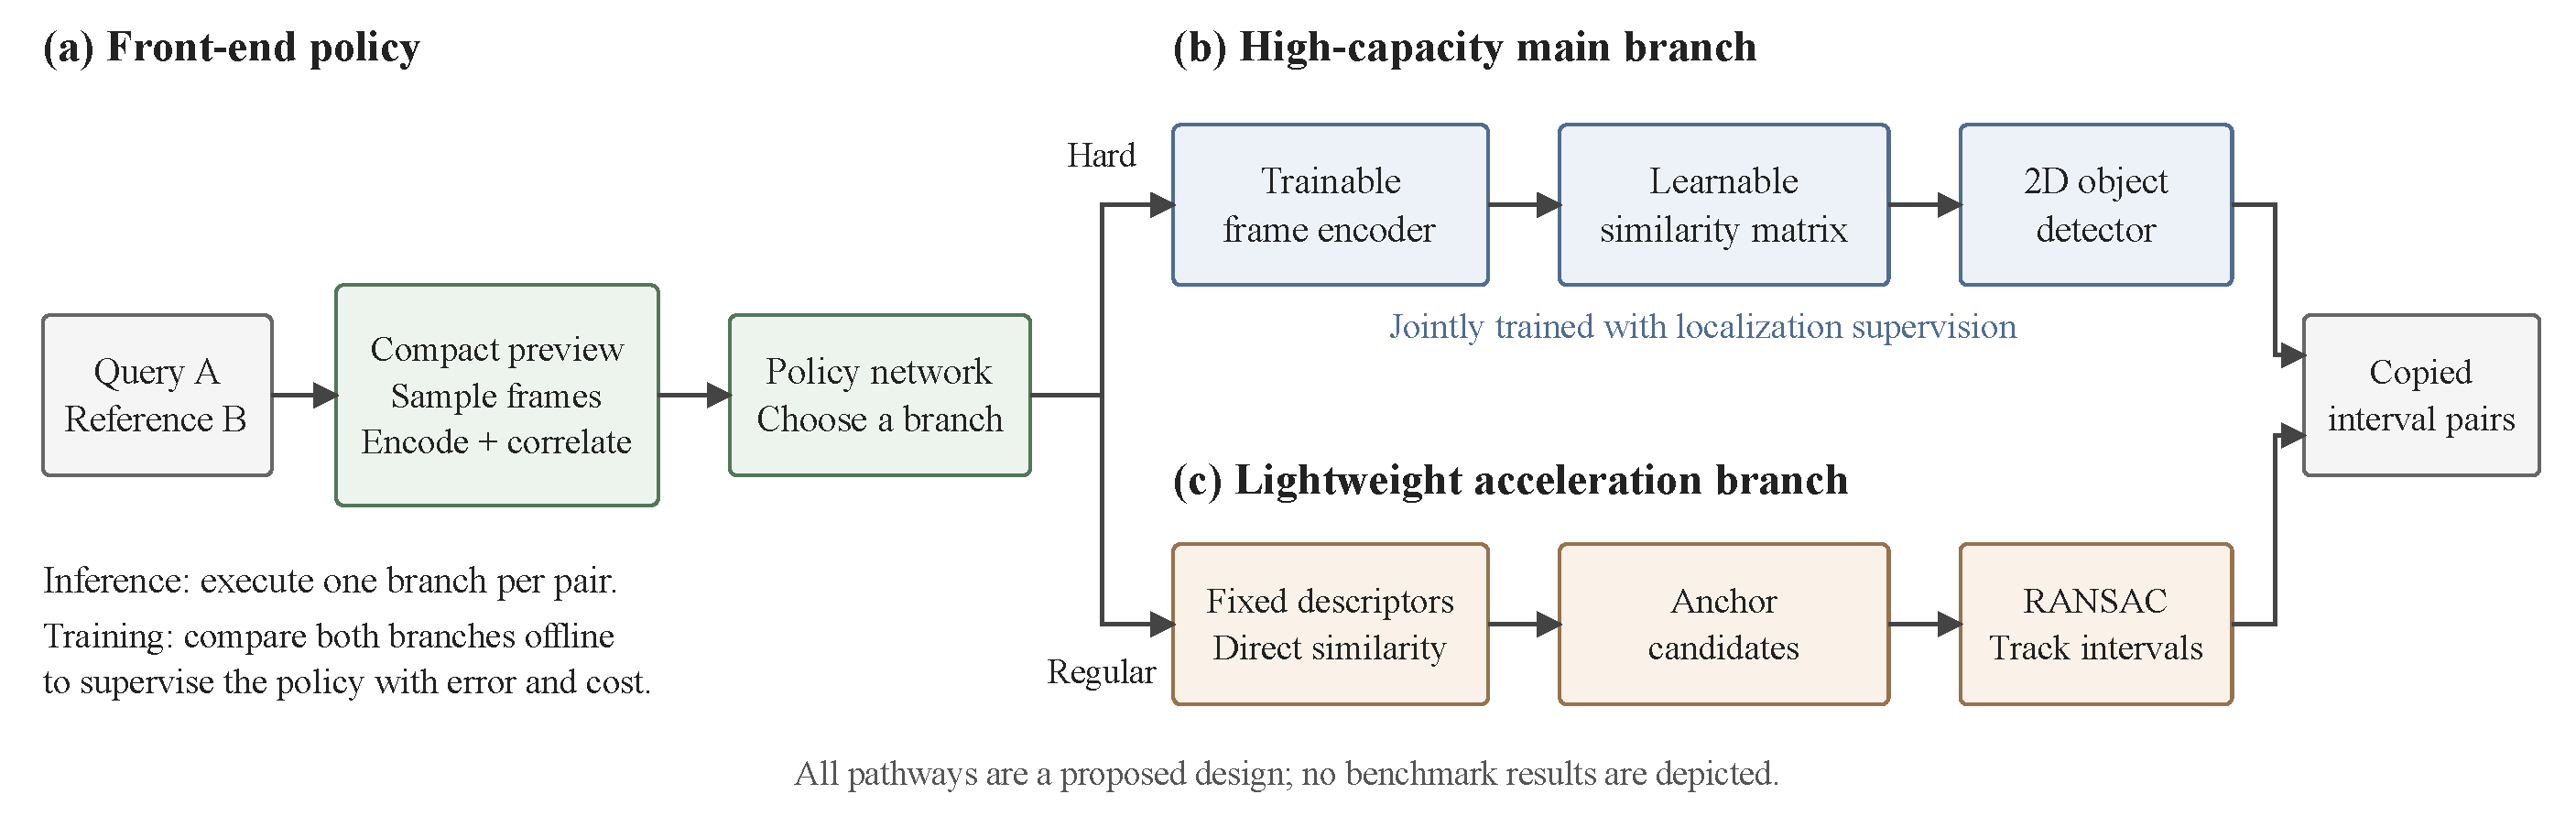
\includegraphics[width=\textwidth]{figures/framework.pdf}
\colorbox{lightgray}{%
  \parbox{\dimexpr\textwidth-2\fboxsep\relax}{%
    \vspace{14pt}\centering
    \textbf{\color{primary}[ Placeholder for \texttt{figures/framework.pdf} ]}\\[4pt]
    \footnotesize (a) Feature Encoder \& Learnable Similarity Matrix with Object Detection $\rightarrow$ (b) Selective Track Recovery $\rightarrow$ (c) Selective Boundary Refinement \& Dual-Axis Deduplication
    \vspace{14pt}%
  }%
}
\caption{\textbf{Overview of FastVCL.} Built upon a frame feature encoder, a learnable similarity matrix, and a candidate tube detector, FastVCL introduces a confidence-aware selective model to resolve the efficiency--accuracy trade-off. (a) A primary detection branch identifies high-precision candidate tracks over the similarity matrix and refines local bands. (b) A shadow proposal pass exposes weak candidate tracks, filtering them through geometric constraints and a selective admission module to recover subtle copies without dense matching. (c) Candidate segments undergo selective discrete boundary refinement revalidated against local similarity features, followed by dual-axis deduplication to preserve one-to-many copy mappings.}
\label{fig:framework}
\end{figure*}

\paragraph{Bridging Similarity Detection and Selective Modeling.}
To break this efficiency--accuracy bottleneck, we observe that not all candidate regions in a similarity matrix require the same computational or decision depth. Clear matches and obvious background pairs can be resolved rapidly by standard sparse similarity detection, whereas ambiguous weak tracks and fuzzy segment endpoints require targeted verification. Motivated by this insight, we propose \textbf{FastVCL}, a fast and accurate VCL framework that integrates a confidence-aware \emph{selective model} directly into the classic feature encoder, learnable similarity matrix, and object detection pipeline (Figure~\ref{fig:framework}). Rather than exhaustively evaluating dense correspondence maps, FastVCL allocates computation selectively across two critical localization bottlenecks: (i) determining whether a weak temporal correspondence is a genuine copy missed by strict detection, and (ii) pinpointing where an admitted copy precisely starts and ends.

\paragraph{Selective Track Recovery and Boundary Refinement.}
Specifically, FastVCL extracts frame descriptors via a visual encoder and constructs a learnable similarity matrix to guide candidate tube detection. A primary high-precision branch identifies confident anchor tracks and refines narrow temporal bands via local alignment. In parallel, a lightweight shadow pass relaxes support constraints over the learned similarity representations to expose weak candidate tracks. Rather than admitting all relaxed proposals—which would severely degrade precision—a hard geometric gate eliminates physically inconsistent trajectories (e.g., invalid temporal slopes, excessive residuals, or structural gaps), and our selective model estimates track-level copy confidence. Following a fail-closed principle, only candidate tracks exceeding a calibrated selective threshold are admitted into the localization tube. Subsequently, for boundary localization, each candidate segment (from either the primary or recovery path) is paired with a compact set of discrete boundary hypotheses (keep, extend left/right/both, or shrink) revalidated against local similarity features. The selective module evaluates these hypotheses and updates the interval only when prediction confidence is high, safely falling back to the initial detector boundary otherwise. Finally, a dual-axis deduplication strategy merges overlapping tubes only when they coincide along both query and reference timelines, ensuring that a single query segment repeated across multiple reference locations is preserved as distinct copy instances.

\paragraph{Why Selective Decisions Over Dense Matching?}
Our design is grounded in a clear empirical observation: indiscriminate densification of the similarity matrix is an inefficient way to buy recall. As shown in our empirical analysis, densifying the anchor grid from stride 4 to 1 more than doubles recall and substantially boosts F1, but simultaneously degrades precision and multiplies inference cost due to false matches on repetitive visual patterns. By coupling a learnable similarity detector with a selective verification and refinement head, FastVCL separates true weak copies from hard negatives at a fraction of the cost of dense matching. Furthermore, because the selective model operates over structured similarity and geometric evidence with a strict fail-closed fallback, it guarantees stable localization without hallucinating unconstrained coordinates.

\paragraph{Contributions.}
In summary, our main contributions are three-fold:
\begin{itemize}
\setlength{\itemsep}{2pt}\setlength{\parskip}{0pt}
    \item \textbf{Selective VCL Architecture:} We propose \textbf{FastVCL}, a unified video copy localization framework that seamlessly couples a frame feature encoder, a learnable similarity matrix, and correspondence-map object detection with a confidence-aware selective model, achieving sub-quadratic efficiency without sacrificing recall.
    \item \textbf{Fail-Closed Track Recovery \& Boundary Refinement:} We design a two-stage selective mechanism comprising shadow track recovery and discrete boundary refinement, complemented by dual-axis deduplication to accurately capture weak, heavily edited, and one-to-many copy instances.
    \item \textbf{State-of-the-Art Speed--Accuracy Trade-off:} Extensive experiments and diagnostic ablations on standard VCL benchmarks demonstrate that FastVCL achieves localization accuracy on par with state-of-the-art dense detectors while delivering a substantial inference speedup.
\end{itemize}
\section{Related Work}
\label{sec:related}

\paragraph{Video copy localization.}
VCDB and VCSL provide segment annotations for partial video copies~\cite{jiang2014,vcsl2022}.
VCL requires temporal intervals rather than only a video-level similarity score. Comparisons
depend on dataset version, negative pairs, descriptors, and the overlap evaluator. SPD studies
copy patterns on similarity maps~\cite{spd2021}. TransVCL combines feature enhancement,
similarity generation, and temporal detection in a jointly optimized network~\cite{transvcl2023}.
Its self- and cross-attention illustrate the value of learning context before localization.
FastVCL retains a learned correspondence-map detector as its main branch and studies when a
pair can use a cheaper geometric branch instead.

\paragraph{Geometric temporal alignment.}
Classical approaches enforce temporal consistency among frame matches, including temporal
networks and pattern-based alignment~\cite{tan2009,chou2015}. VCSL compares Hough voting,
temporal networks, dynamic programming, and dynamic time warping alongside learned
detection~\cite{vcsl2022}. Our acceleration branch uses RANSAC~\cite{fischler1981} to fit affine
temporal tracks from direct descriptor matches. Such tracks suit regular correspondences,
but a single track cannot represent arbitrary reordering or discontinuous editing. A separate
learned pathway accommodates more complex pairs. We evaluate branch selection rather than
assuming geometric alignment is sufficient for all inputs.

\paragraph{Dynamic computation and policy networks.}
BlockDrop learns input-dependent choices of residual blocks through a policy that trades
recognition quality against computation~\cite{wu2018blockdrop}. SkipNet learns to skip
convolutional blocks using intermediate activations to guide dynamic routing~\cite{wang2018skipnet}.
These methods motivate adapting computation to the input. FastVCL applies this principle to
pairwise localization and selects between two mechanisms: learned detection and geometric
alignment. Routing occurs before either complete localizer runs. Its supervision accounts
for missed segments, false copies, and boundary error, rather than classification alone.

\paragraph{Positioning.}
A faster detector, a sparser matcher, and a learned router address different sources of cost.
Their combination alone does not establish an advantage. Always-main and always-acceleration
baselines isolate branch quality; matched-utilization routing controls isolate the policy;
and measurements including preview, feature extraction, and post-processing test whether
conditional execution provides a net benefit.

\section{Method}
\label{sec:method}

\subsection{Problem formulation and architecture}
Given sampled videos $A=(a_i)_{i=0}^{M-1}$ and $B=(b_j)_{j=0}^{N-1}$, the output is a set
$\mathcal S=\{([a_s,a_e),[b_s,b_e),q)\}$ of scored interval pairs. Endpoints satisfy
$0\le a_s<a_e\le M$ and $0\le b_s<b_e\le N$ on the original sampled timelines. A timestamp
map converts indices to video time. An empty set denotes no detected copy; multiple intervals
can represent repeated copies.

FastVCL has a policy $\pi_\theta$, a main localizer $\mathcal F_{\rm m}$, and an acceleration
localizer $\mathcal F_{\rm a}$. For a compact preview $z(A,B)$, the policy produces
$p_{\rm m}=\pi_\theta(z)\in[0,1]$. With validation-selected threshold $\eta$,
\begin{equation}
r=\mathbb{1}[p_{\rm m}\ge\eta],\qquad
\mathcal S=\begin{cases}
\mathcal F_{\rm m}(A,B),&r=1,\\
\mathcal F_{\rm a}(A,B),&r=0.
\end{cases}
\label{eq:route}
\end{equation}
Only one localizer executes per pair at inference. A missing or non-finite policy score
selects the main branch and is logged. A valid low score selects acceleration even if it
subsequently finds no anchors; there is no unreported second main-branch pass. The following
specifies the proposed network and training procedure, not an already trained implementation.

\subsection{Front-end policy network}
\label{sec:policy}
\paragraph{A bounded preview.}
The policy uniformly samples at most $K$ low-resolution frames per video. A lightweight
encoder $\psi_\phi$ produces normalized descriptors $u_i,v_j\in\mathbb R^{d_p}$.
Short videos are padded with validity masks. From the small map $C_{ij}=u_i^\top v_j$,
we form
\begin{equation}
z=\bigl[\operatorname{pool}(U),\operatorname{pool}(V),
\operatorname{vec}(\widetilde C),\ell_A,\ell_B\bigr],
\label{eq:preview}
\end{equation}
where pooling is a masked temporal mean, $\widetilde C$ contains the masked correlation map
and its validity mask, and $\ell_A=\log(1+M)$, $\ell_B=\log(1+N)$. An MLP followed by a
sigmoid produces $p_{\rm m}$. The ordered correlation map retains coarse continuity and
competing matches that pooled video descriptors alone would discard. Its size is bounded
by $K^2$, independently of $MN$.

The preview uses neither ground truth nor full-localizer outputs at inference. In particular,
the main similarity map is not computed to decide whether to skip it. Preview decoding,
including seeking into compressed videos, is part of routing overhead. The supplement gives
an initial design for $K$, resolution, encoder, and MLP; these choices remain to be validated.

\paragraph{Reference policy instantiation.}
The initial design uses $K=16$ frames at $112\times112$, three stride-2 convolution
layers with 32/64/128 channels, ReLU, and spatial mean pooling. Two temporal means,
the correlation map and mask, and two lengths give 770 inputs to a $770\to128\to1$ MLP.
These are reproducible starting dimensions, not measured optima; capacity ablations
include each variant's preview cost.

\paragraph{Learning branch preference.}
Let $\ell_b(A,B)$ be branch $b$'s localization error against training annotations and let
$c_b(A,B)$ be its profiled cost divided by a fixed positive reference cost,
$b\in\{{\rm m},{\rm a}\}$. Both branches use the same error definition, penalizing missed
copies, unmatched predictions, and interval misalignment (supplement).
For completeness, let $P_b$ be a branch's predictions and $G$ the annotated interval pairs.
Define $u(p,g)=\min\{\mathrm{IoU}_A(p,g),\mathrm{IoU}_B(p,g)\}$ and form a one-to-one
matching $\mathcal M_b$ over pairs with $u\ge0.5$, maximizing cardinality first and total
agreement second. With unmatched prediction and annotation counts $U_P,U_G$, we use
\begin{equation}
\ell_b=\frac{U_P+U_G+\sum_{(p,g)\in\mathcal M_b}(1-u(p,g))}
{\max(1,|P_b|+|G|)}.
\label{eq:branch-error}
\end{equation}
The normalization bounds $\ell_b$ in $[0,1]$. Correctly returning no copies on a negative
pair gives zero error; missing every annotated copy or returning any copies on a negative
pair gives one. The matching term distinguishes accurate intervals from marginal matches.
This is a common training surrogate for comparing branches, not a replacement for the
benchmark evaluator. In particular, its treatment of negative pairs emphasizes whether a
false alarm occurs, while the evaluation also records the number of false copies.
Offline evaluations define
\begin{equation}
y^*=\mathbb{1}\!\left[\ell_{\rm m}+\lambda c_{\rm m}
<\ell_{\rm a}+\lambda c_{\rm a}\right],
\label{eq:policy-target}
\end{equation}
where $\lambda\ge0$ controls the cost penalty and ties select acceleration. The policy and
preview encoder minimize binary cross-entropy:
\begin{equation}
\mathcal L_{\rm policy}=-y^*\log p_{\rm m}-(1-y^*)\log(1-p_{\rm m}).
\label{eq:policy-loss}
\end{equation}
Targets use frozen branch checkpoints on a held-out portion of the training split, avoiding
in-sample estimates from the main branch's fitting data. Costs may depend on sequence length
and are profiled on training data. Validation selects $\lambda$ and $\eta$ for the desired
accuracy--latency operating point. The score predicts branch preference, not a calibrated
probability that a pair contains a copy.

\paragraph{What a routing mistake costs.}
Define the per-pair branch objective $J_b=\ell_b+\lambda c_b$ and margin
$\Delta=J_{\rm a}-J_{\rm m}$. The target in Eq.~\ref{eq:policy-target} selects main exactly
when $\Delta>0$. For any binary routing action $r$, the excess objective is
\begin{equation}
J_{r}-\min(J_{\rm m},J_{\rm a})
=|\Delta|\,\mathbb{1}[r\ne y^*],
\label{eq:regret}
\end{equation}
where $J_r=rJ_{\rm m}+(1-r)J_{\rm a}$. This identity follows by considering the sign of
$\Delta$; ties have zero regret. It explains why routing accuracy alone is insufficient:
choosing the wrong branch on an almost indifferent pair matters less than missing a pair
where main substantially improves localization. The reference policy uses unweighted
cross-entropy, while evaluation reports both action error and objective regret. A policy
with high action accuracy can still be poor if its errors concentrate on large-margin
pairs. The margin is available only during offline supervision or analysis; the deployed
policy must infer branch preference from the preview.

\subsection{High-capacity main branch}
\label{sec:main-branch}
\paragraph{Trainable representations and similarity.}
The main encoder $\Phi_\omega$ maps frames to $F^A,F^B$. A trainable interaction module
$G_\xi$ adds temporal context and exchanges information across sequences, producing
$H^A,H^B$. Learned projections give normalized vectors $\widehat h_i^A,\widehat h_j^B$
and the differentiable affinity
\begin{equation}
S^{\rm m}_{ij}=\operatorname{sigmoid}
\bigl(\kappa(\widehat h_i^A)^\top\widehat h_j^B+b_0\bigr),
\label{eq:main-sim}
\end{equation}
with learned positive scale $\kappa$ and bias $b_0$. The main branch adapts representations
and correspondence scores to localization supervision and processes the full valid
correspondence domain; padded cells are masked.

\paragraph{Correspondence structure and repeated copies.}
The learned map differs from direct cosine matching in two places: temporal interaction
changes the descriptors using surrounding frames, and localization gradients adapt their
projections and affinity scale. Thus a locally ambiguous frame can be interpreted in the
context of its neighboring sequence. The elementwise sigmoid does not normalize each row
into a mutually exclusive distribution over reference frames. This allows one query frame
to support several separated reference occurrences, an important possibility when a clip
is repeated. The map alone does not guarantee that the detector returns every occurrence;
that depends on training, output thresholds, and suppression.

An annotated interval rectangle is not treated as a dense matrix of positive frame matches.
Its interior contains frame pairs at different relative times, most of which need not
correspond. We therefore train the map through the interval detector rather than labeling
every cell inside a copied rectangle as positive. This preserves the distinction between
segment supervision and exact alignment supervision.

\paragraph{2D detection of copied intervals.}
A convolutional detector $D_\nu$ consumes $S^{\rm m}$ and predicts objectness and rectangles.
Query time is the vertical axis and reference time the horizontal axis. A normalized box
$(x_s,y_s,x_e,y_e)$ decodes to $[My_s,My_e)\times[Nx_s,Nx_e)$ before conversion to valid
timeline endpoints. Multiple boxes represent multiple copies. A rectangle specifies the
intervals without requiring a single affine frame correspondence throughout its interior.

Training matches predicted boxes to annotated intervals and combines objectness loss,
normalized endpoint regression, and generalized box IoU loss~\cite{rezatofighi2019giou}:
\begin{equation}
\mathcal L_{\rm main}=\mathcal L_{\rm obj}
+\lambda_{\rm box}\mathcal L_1+\lambda_{\rm iou}\mathcal L_{\rm GIoU}.
\label{eq:main-loss}
\end{equation}
Regression applies to matched boxes; unmatched detector locations receive background
objectness targets. Gradients pass through the detector, similarity module, interaction module,
and frame encoder, making this branch end-to-end trainable. Segment labels supervise boxes,
not dense frame correspondence. Cached-feature experiments must be reported separately
because they cannot train the image encoder end to end.

\paragraph{Assignment and negative pairs.}
One-to-one assignment minimizes a fixed combination of normalized endpoint distance
and generalized IoU cost. Matched predictions receive positive objectness targets and
box supervision; unmatched predictions receive background targets. Negative pairs have
zero regression loss. Normalize box losses by at least one matched instance, record
objectness normalization separately, and freeze assignment weights across comparisons.
This training assignment does not replace the benchmark's independent evaluator.

\subsection{Lightweight acceleration branch}
\label{sec:acceleration}
\paragraph{Direct similarity and anchors.}
A fixed pretrained encoder $\Phi_{\rm a}$, or its cached features, provides normalized
descriptors without the main interaction module. Their direct cosine similarity is
$S^{\rm a}_{ij}=(f_i^A)^\top f_j^B$. For stride $s$, grids
$I_s=\{0,s,2s,\ldots\}\cap[0,M)$ and $J_s$ define the evaluated frame pairs. Anchors are
mutual top-1 matches exceeding $\tau_{\rm anc}$:
\begin{equation}
\begin{split}
\mathcal A=\{(i,j):\;&j=\argmax_{v\in J_s}S^{\rm a}_{iv},\quad
i=\argmax_{u\in I_s}S^{\rm a}_{uj},\\
&S^{\rm a}_{ij}\ge\tau_{\rm anc}\}.
\end{split}
\label{eq:anchors}
\end{equation}
Ties use the smaller timeline index. Tiled computation maintains row and column maxima
without storing the complete map. Grid subsampling reduces similarity evaluations; it does
not retroactively reduce feature-extraction cost for already cached descriptors.

\paragraph{RANSAC temporal alignment.}
RANSAC fits $j=\sigma i+\beta$. A track needs at least $n_{\min}$ inliers, slope in
$[\sigma_{\min},\sigma_{\max}]$, and residuals at most $\epsilon$. Accepted inliers are
removed before searching for another track. Within a track, anchors are sorted by query time
and split at gaps above $g_{\max}$ or violations of reference ordering. Supported runs yield
intervals from their first and last matched indices, with an exclusive upper endpoint one
sample beyond the last match.

A bounded endpoint check searches at most $s-1$ unsampled query positions beyond each end,
following the fitted line within residual tolerance. Extension stops when no valid reference
match reaches $\tau_{\rm anc}$ or an axis limit is reached. Reference endpoints are updated
from the accepted matches, whose mean cosine supplies the segment score. This local check
reduces sampling imprecision but cannot guarantee exact endpoints. No 2D detector, learned
similarity head, or dynamic program runs in this branch.

Segments must meet minimum duration and support constraints on both timelines. Duplicate
suppression retains the higher-score segment only when query IoU and reference IoU both
exceed $\tau_{\rm dup}$. The same interval-validity and duplicate rules apply to main outputs.
Disjoint reference occurrences of the same query interval can therefore survive, subject to
the output cap. Predictions come from the selected branch only; scores are not fused across
pathways.

\begin{algorithm}[t]
\caption{FastVCL inference for one video pair}
\label{alg:inference}
\begin{algorithmic}[1]
\Require Videos $A,B$; trained policy and main branch; fixed acceleration settings; threshold $\eta$
\Ensure Scored interval pairs $\mathcal S$ and selected route $r$
\State $z\gets\operatorname{Preview}(A,B)$
\State $p_{\rm m}\gets\pi_\theta(z)$
\If{$p_{\rm m}$ is missing or non-finite}
    \State $r\gets1$; record policy fallback
\Else
    \State $r\gets\mathbb{1}[p_{\rm m}\ge\eta]$
\EndIf
\If{$r=1$}
    \State $(F^A,F^B)\gets\Phi_\omega(A,B)$
    \State $S^{\rm m}\gets\operatorname{LearnedSimilarity}(G_\xi(F^A,F^B))$
    \State $\mathcal P\gets\operatorname{DecodeBoxes}(D_\nu(S^{\rm m}))$
\Else
    \State $(f^A,f^B)\gets\Phi_{\rm a}(A,B)$
    \State $\mathcal A\gets\operatorname{MutualAnchors}(f^A,f^B,s,\tau_{\rm anc})$
    \State $\mathcal T\gets\operatorname{RANSACTracks}(\mathcal A)$
    \State $\mathcal P\gets\operatorname{SplitAndCheckEndpoints}(\mathcal T,f^A,f^B)$
\EndIf
\State $\mathcal S\gets\operatorname{ValidateAndDeduplicate}(\mathcal P)$
\State \Return $(\mathcal S,r)$
\end{algorithmic}
\end{algorithm}

\subsection{Training schedule and inference cost}
\label{sec:cost}
First, optimize the main localizer and fix the acceleration configuration and branch-specific
output-score thresholds using validation data. Second, freeze both branches, generate
preference targets on held-out training pairs, and train the policy. Third, select the policy
threshold on validation data, then freeze the system for testing. A subsequent change to a
branch checkpoint or score threshold requires regenerating the policy targets: the detector's
objectness and the acceleration branch's cosine score are not interchangeable, and changing
their cutoffs changes both errors in Eq.~\ref{eq:policy-target}. Both branches run offline
to generate targets, but only the selected branch runs at inference
(Algorithm~\ref{alg:inference}). No gradient through RANSAC or the routing action is required.

For pair $x$, let $T_{\rm p}$ include preview construction and policy inference,
$T_{\rm m},T_{\rm a}$ include branch features and localization, and $T_{\rm out}$ include
final interval conversion and serialization:
\begin{equation}
T(x)=T_{\rm p}(x)+r(x)T_{\rm m}(x)
+(1-r(x))T_{\rm a}(x)+T_{\rm out}(x).
\label{eq:cost}
\end{equation}
With main utilization $\rho=\Pr(r=1)$, expected branch cost is
$\rho\,\mathbb E[T_{\rm m}\mid r=1]+(1-\rho)\mathbb E[T_{\rm a}\mid r=0]$.
Conditional means matter because routing can depend on length and difficulty.
Savings over always-main require
\begin{equation}
\mathbb E[(1-r)(T_{\rm m}-T_{\rm a})]>\mathbb E[T_{\rm p}]
\label{eq:break-even}
\end{equation}
under identical input/output accounting. Accurate routing alone does not guarantee speedup.

The preview map has at most $K^2$ cells; the acceleration grid has
$\lceil M/s\rceil\lceil N/s\rceil$ cells. Main matching remains dense. For fixed $s$,
acceleration matching is still $O(MN)$: FastVCL targets lower expected runtime through
conditional computation and smaller constants, not a sub-quadratic worst-case bound.
End-to-end speedup must include the actual branch encoders and decoding.

\paragraph{Matching memory and track overhead.}
Let $M_s=\lceil M/s\rceil$, $N_s=\lceil N/s\rceil$, and use similarity tiles of size
$b_A\times b_B$. Maintaining each row's and column's best score and index requires
$O(M_s+N_s)$ auxiliary storage, so matching workspace is
$O(b_A b_B+M_s+N_s)$ excluding descriptors. Mutual matching is recovered after all tiles
have been visited. This reduces peak map memory without reducing the total number of
similarities. If $I$ RANSAC trials inspect at most $|\mathcal A|$ anchors for each of
$R$ retained tracks, a conservative fitting bound is $O(RI|\mathcal A|)$.
Accordingly, track caps and tile dimensions must be reported alongside stride; a smaller
map alone does not describe the acceleration branch's full resource use.

\section{Experiments}
\label{sec:exp}

\subsection{Evaluation protocol and evidence status}
The evaluation targets VCSL and VCDB~\cite{vcsl2022,jiang2014}. For each benchmark, training,
validation, and test pairs must follow a frozen split manifest, with related video identities
kept together when creating the policy's held-out training partition. Validation selects
routing, matching, and output thresholds; test annotations are reserved for final reporting.
Dataset revisions and added negative pairs must be identified explicitly.

\paragraph{Current evidence.}
The available experiment records describe an earlier geometric localizer with fixed ISC
features. They contain no trained front-end policy, end-to-end main branch, or evaluation
of the present dual-pathway system. Tables~\ref{tab:main}--\ref{tab:ablation} therefore specify
the required comparisons and have no measured new-system results. In particular, comparable
state-of-the-art accuracy and significant speedup, as stated in the abstract, remain to be
substantiated by these runs. Historical values in Section~\ref{sec:history} are preserved as
diagnostics and are not substituted into new-system cells.

\paragraph{Accuracy and boundary metrics.}
The primary report uses each benchmark's official evaluator and aggregation, recording its
version and options. VCSL copy-overlap precision, recall, and F1 must not be relabeled as
pair-classification accuracy or replaced by a different tIoU rule. As a separate diagnostic,
one-to-one segment matching requires IoU of at least $0.5$ on each timeline; a stricter
$0.7$ variant is reported separately. On matched segments, we report mean absolute error
over all four endpoints and the fraction with all endpoints within one, two, and four
sampled frames. These are conditional boundary statistics, accompanied by segment recall
so that missing difficult copies cannot improve them invisibly.

Negative-pair false-alarm rate is the fraction of annotated negative pairs receiving any
prediction. Multi-copy recall counts individually matched annotated instances. Routing
statistics include main utilization $\rho$, branch-conditioned quality, and the error increase
relative to selecting the lower-error branch offline. Both positive and negative pairs are
included; error events such as timeouts or out-of-memory failures are recorded separately
rather than converted to empty predictions.

\paragraph{Timing and resource accounting.}
Primary latency is measured from input decoding through output serialization at batch size
one on the same hardware and precision. We record mean, median, and 95th-percentile latency,
throughput, peak device memory, and the components in Eq.~\ref{eq:cost}. GPU timing uses
synchronization, documented warm-up, and repeated runs. A separate cached-feature experiment
can isolate localization overhead, but its speedup is labeled accordingly. Both branch
encoders and the policy preview are included in end-to-end measurements. Cache reuse,
video decoding, input resolution, and sequence-length limits must be identical or explicitly
accounted for in comparisons.

\subsection{Main comparison}
We compare geometric baselines (HV, TN, DP, and DTW), correspondence-map detection (SPD and
TransVCL), always-main, always-acceleration, and policy-guided FastVCL. Baselines require
controlled reruns under the same split and evaluator; published values from other settings
are not directly combined with new measurements. The always-main and always-acceleration
systems use exactly the branch checkpoints/configurations used by the routed system and
omit the unused policy. This comparison tests whether routing improves the achievable
accuracy--latency operating point.

\begin{table*}[t]
\centering\small
\setlength{\tabcolsep}{6pt}
\caption{Planned main comparison. $P$, $R$, and F1 use the corresponding benchmark's official
evaluator. Mean latency includes decoding, features, routing when applicable, localization,
and output. Every dash is an unmeasured result, not zero. No row in this table has been run
under the proposed protocol.}
\label{tab:main}
\begin{tabular}{@{}lcccccccc@{}}
\toprule
& \multicolumn{4}{c}{VCSL} & \multicolumn{4}{c}{VCDB}\\
\cmidrule(lr){2-5}\cmidrule(lr){6-9}
Method & $P$ & $R$ & F1 & ms/pair & $P$ & $R$ & F1 & ms/pair\\
\midrule
HV / TN / DP / DTW (each) & -- & -- & -- & -- & -- & -- & -- & --\\
SPD & -- & -- & -- & -- & -- & -- & -- & --\\
TransVCL & -- & -- & -- & -- & -- & -- & -- & --\\
FastVCL always-main & -- & -- & -- & -- & -- & -- & -- & --\\
FastVCL always-acceleration & -- & -- & -- & -- & -- & -- & -- & --\\
FastVCL policy-guided & -- & -- & -- & -- & -- & -- & -- & --\\
\bottomrule
\end{tabular}
\end{table*}

\subsection{Routing and component ablations}
\paragraph{Does the policy select the right pairs?}
Table~\ref{tab:routing} compares learned routing with two controls at matched main utilization.
Random routing selects pairs without looking at their contents and is repeated over seeds.
A deterministic rule uses preview-correlation ambiguity (the mean gap between the largest
and second-largest valid row similarities), routing ambiguous pairs to the main branch.
Its threshold is selected on validation data. Both controls include the same preview cost
for the policy-isolation comparison; a random router without the preview is additionally
timed as a deployment control.

An offline oracle chooses the lower error-plus-cost branch for each pair using ground truth.
It is a diagnostic reference for routing regret, not an executable test-time method or a
latency result. Sweeping $\eta$ traces the measured accuracy--latency curve; selection of a
reported operating point is confined to validation. A useful policy should improve quality
over matched-utilization controls and beat always-main latency after including its overhead.

\begin{table}[t]
\centering\footnotesize
\setlength{\tabcolsep}{4pt}
\caption{Routing comparison on VCSL (pending). $\rho$ is main-branch utilization; regret is
mean excess localization error over the lower-error branch. Fixed utilization for the
always-branch rows is structural, not measured.}
\label{tab:routing}
\begin{tabular}{@{}lcccc@{}}
\toprule
Routing & $\rho$ & F1 & ms/pair & regret\\
\midrule
Always-main & 1 & -- & -- & --\\
Always-acceleration & 0 & -- & -- & --\\
Random, matched $\rho$ & -- & -- & -- & --\\
Preview rule, matched $\rho$ & -- & -- & -- & --\\
Learned policy & -- & -- & -- & --\\
\bottomrule
\end{tabular}
\end{table}

\paragraph{Which components matter?}
Table~\ref{tab:ablation} defines independent changes to the proposed system. Removing the
ordered correlation preview tests whether global appearance alone predicts branch difficulty.
Removing the cost term tests whether quality-only supervision overuses the main branch.
Freezing the main encoder isolates adaptation of frame features; replacing learned similarity
with direct cosine isolates correspondence learning. Removing RANSAC replaces geometric
verification with contiguous monotone runs of mutual matches. Disabling the endpoint check
measures the cost and boundary contribution of local resampling. Branch modifications use
the same training partition and regenerate policy targets; a separately reported frozen-policy
evaluation can reveal sensitivity to branch changes.

\begin{table}[t]
\centering\footnotesize
\setlength{\tabcolsep}{3pt}
\caption{Component ablations on VCSL (pending). Each row changes one component from full
FastVCL. MAE is four-endpoint mean absolute error on matched instances, in sampled frames.}
\label{tab:ablation}
\begin{tabular}{@{}lcccc@{}}
\toprule
Variant & F1 & MAE & $\rho$ & ms/pair\\
\midrule
Full policy-guided system & -- & -- & -- & --\\
Pooled preview only & -- & -- & -- & --\\
Quality-only policy ($\lambda=0$) & -- & -- & -- & --\\
Frozen main encoder & -- & -- & -- & --\\
Direct cosine in main branch & -- & -- & -- & --\\
Acceleration without RANSAC & -- & -- & -- & --\\
Acceleration without endpoint check & -- & -- & -- & --\\
\bottomrule
\end{tabular}
\end{table}

\subsection{Historical anchor diagnostics}
\label{sec:history}
The frozen workbook contains 25 reported runs of an earlier fixed-feature system on the VCSL
test split. Table~\ref{tab:history} preserves selected values; the supplement transcribes all
25 rows. Prediction files, run configurations, and evaluation logs have not been reconciled
for every row. Values are therefore historical reported metrics, not controlled reruns of
the proposed branches. Most selected rows include a tube and dynamic program, which the
new acceleration pathway does not use.

\begin{table}[t]
\centering\footnotesize
\setlength{\tabcolsep}{4pt}
\caption{Historical VCSL diagnostics from the workbook, in percent. Row IDs retain provenance.
Rows are not results of the current main branch, acceleration branch, or policy.}
\label{tab:history}
\begin{tabular}{@{}rlrrr@{}}
\toprule
Row & Configuration & $P$ & $R$ & F1\\
\midrule
13 & Strict, stride 4, inliers 5 & 93.94 & 14.36 & 24.91\\
21 & Stride 2 & 89.04 & 25.96 & 40.20\\
22 & Stride 1 & 86.33 & 31.15 & 45.79\\
23 & Inliers 3 & 89.93 & 21.97 & 35.31\\
24 & Inliers 2 & 89.13 & 24.07 & 37.90\\
15 & No DP, argmax & 85.11 & 16.53 & 27.68\\
17 & Direct track-to-segment & 94.05 & 13.69 & 23.90\\
33 & Argmax, relaxed anchors & 63.58 & 56.23 & 59.68\\
\bottomrule
\end{tabular}
\end{table}

The strict recorded setting is precision-heavy and recall-poor. Densifying its anchor grid
from stride 4 to 1 changes recall from 14.36 to 31.15 and precision from 93.94 to 86.33.
Reducing the inlier requirement also increases recall. Row 33 changes several settings
together and cannot isolate the effect of replacing DP. These observations suggest that
one geometric operating point is unlikely to suit every pair. They do not show which pairs
a learned policy would route correctly. Workbook elapsed times have ambiguous scope and
hardware provenance, so they are not used to calculate an inference speedup.

\subsection{Failure analysis and validity}
We stratify results by copy duration, speed change, edit severity, repeated content, and
sequence length wherever annotations support those categories. The main questions are whether
the preview misses short copies, whether regular pairs receive unnecessary main computation,
and whether acceleration increases false alarms on repetitive backgrounds. Qualitative
examples must include routing failures and both branches' offline predictions, with the
latter clearly distinguished from deployed computation.

A speedup claim requires measured net latency savings, and competitive accuracy requires a
controlled comparison at the same evaluator and split. Neither follows from historical
anchor diagnostics. Policy errors may shift under new editing styles or duration distributions.
Cached features cannot substantiate end-to-end encoder training or raw-video latency.
Exact endpoints also depend on the sampling rate and timestamp map. These limits remain
until the pending training and benchmark runs are completed.

\section{Conclusion and Limitations}
\label{sec:conclusion}
FastVCL allocates computation at the video-pair level. A lightweight front-end policy chooses
between an end-to-end trainable main branch with learned similarity and 2D detection, and an
acceleration branch using direct similarity, anchors, and RANSAC temporal alignment.
Cost-aware supervision and a validation-selected threshold define the intended
accuracy--efficiency operating point. Only the selected branch executes at inference, so
potential savings depend on avoided computation exceeding routing overhead.

A compact preview can miss short copies and route a difficult pair to acceleration.
Affine tracks can fail under discontinuous edits, and fixed-stride matching remains quadratic
in sequence lengths. Feature extraction, decoding, and policy inference may dominate the
savings from bypassing detection. Historical diagnostics motivate adaptive routing but do
not evaluate the proposed network. Training the policy and main branch, completing controlled
VCSL/VCDB comparisons, and measuring end-to-end latency remain necessary to establish its
accuracy and speedup claims.


{
    \small
    \bibliographystyle{ieeenat_fullname}
    \bibliography{main}
}

% The supplementary material is a separate entry point (supplementary.tex) so
% that detailed audit material stays outside the main paper. Do not \input it here.

% Mandatory LLM usage statement.  The CVPR 2027 guidelines allow the eight-page
% body to be followed by references and this statement on extra pages.
\clearpage
\section*{LLM Usage Statement}
Large language model (LLM) tools assisted with manuscript restructuring,
\LaTeX{} editing, formulation of the policy-guided architecture and evaluation
protocol, figure-generation code, and consistency checks. They were not used to
generate experimental measurements. Historical metrics were transcribed from
existing records; results for the proposed dual-pathway network remain pending.
The proposed training choices require implementation and empirical validation.
The authors are responsible for reviewing the technical content and verifying
all claims before submission.

\end{document}
